\chapter{Metodologia}
\label{cap:03}

O processo de desenvolvimento de um jogo pode ser realizado de diversas formas, dependendo do tipo de jogo a ser criado. Neste trabalho, o desenvolvimento será baseado no diagrama apresentado na figura~\ref{fig:metodologia}, que apresenta todas as etapas do processo de criação do jogo proposto.

\FloatBarrier 
\begin{figure}[!htbp]
	\centering
	\caption{\textit{Diagrama de metodologia}}
	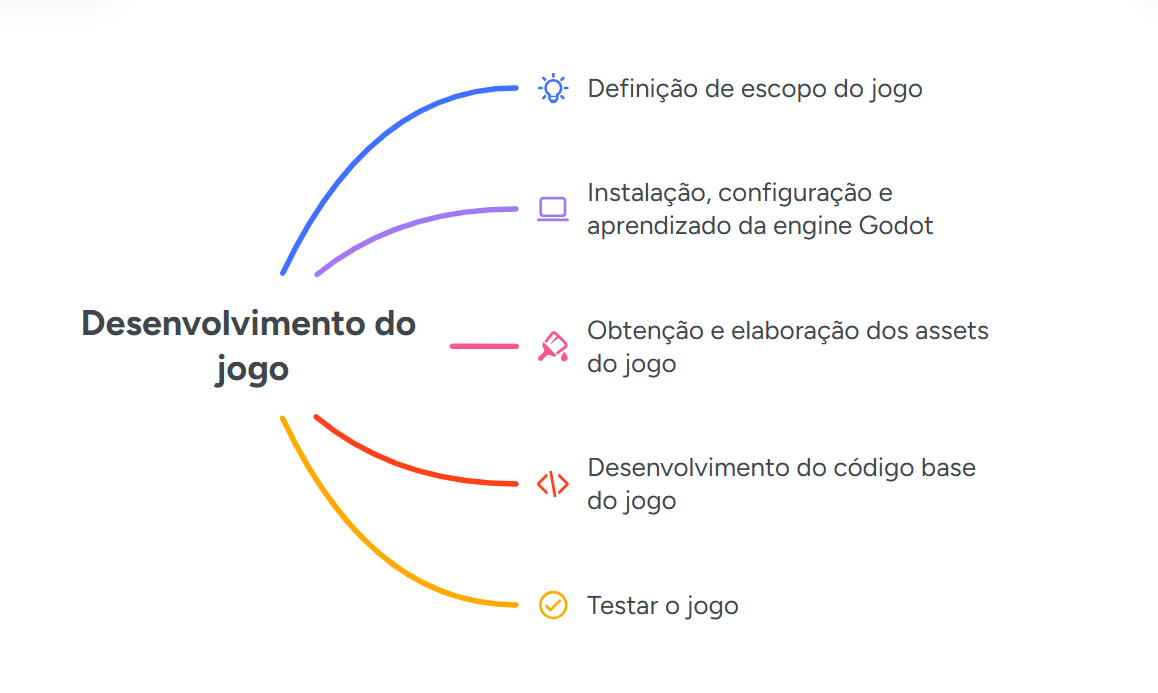
\includegraphics[width=1 \linewidth]{imagens/metodologia.png}
	\\\textbf{Fonte:} Elaborada pelo autor
	\label{fig:metodologia}
\end{figure}
\FloatBarrier


\section{Definição do escopo do jogo}

A definição do escopo uma etapa primordial no desenvolvimento de qualquer jogo, pois orienta as demais fases do projeto. Nessa etapa, será definido o gênero do jogo que será criado e, a partir disso, serão elaboradas as mecânicas, os elementos visuais e demais componentes que darão forma à experiência do jogador. Neste trabalho optou-se pelo desenvolvimento de um \textit{cozy game} em 2D, com o objetivo de proporcionar uma experiência relaxante e acolhedora ao jogador.	

\section{Processo de Instalação, Configuração e Aprendizado da Engine Godot}

O ambiente de desenvolvimento será preparado com o objetivo de tornar o processo mais eficiente em todas as etapas do projeto. Para isso, será escolhida a \textit{Godot Engine}, que se mostra uma boa opção por ser de fácil aprendizado e gratuita. A configuração envolve a instalação da \textit{engine}, a organização das pastas do projeto e o estudo da linguagem \textit{GDScript}. Essa organização inicial busca evitar problemas ao longo da criação do jogo.


\section{Elaboração do Game Design Document (GDD)}




\section{Obtenção e desenvolvimento dos assets do jogo}

Os \textit{assets} são todos os recursos que serão 	utilizados na construção do jogo, podendo ser imagens, efeitos sonoros e músicas. Os \textit{sprites}, elementos básicos que foram utilizados para representar o personagem principal, dando efeito de animação ao mesmo, e para compor o cenário, serão obtidos gratuitamente através do site \textit{itch.io}. Além disso, serão elaborados outros \textit{sprites} para complementar o projeto.

\section{Desenvolvimento do código-base do jogo}

No desenvolvimento do código-base do jogo, serão implementadas as mecânicas principais do personagem, a interface do usuário e outras funcionalidades essenciais para a execução do jogo. Além disso, nessa etapa ocorre a integração dos elementos visuais e sonoros, dando ao jogo uma atmosfera mais coerente e funcional.

\section{Testar o jogo}

Por fim, há a necessidade de realizar testes em todas as funções do jogo, garantido que não haja nenhum \textit{bug} ou erro no código que comprometa a execução do jogo. Também será verificado se todos os requisitos foram atendidos e o jogo funciona conforme o esperado.